%Based on the Amrita Vishwa Vidyapeetham thesis template (Dept. of Artificial Intelligence)

\documentclass[a4paper, 12pt]{report}
\usepackage[margin=0.8in]{geometry}

\usepackage{bold-extra}
\usepackage{amsmath}
\usepackage{amsfonts}
\usepackage{amssymb}
\usepackage{graphicx}
\usepackage [english]{babel}
\usepackage [autostyle, english = american]{csquotes}
\MakeOuterQuote{"}
\usepackage{setspace}
\onehalfspacing
\graphicspath{{images/}}
\usepackage{amsthm}
\usepackage{array}
\usepackage{cite}
\usepackage{longtable}
\usepackage{fancyhdr}
\usepackage{titletoc}
\usepackage{booktabs}
\usepackage{tabularx}
\usepackage{tikz}
\usetikzlibrary{positioning}
\usepackage{microtype}
\usepackage{url}
\theoremstyle{definition}
\newtheorem{Definition}{Definition}[section]
\emergencystretch=3em
\setlength{\parskip}{3pt}

\begin{document}
	\pagenumbering{gobble}
	\thispagestyle{empty}
	\begin{large}
		\begin{center}
			{\Large\bfseries{PROCUREGUARD-AI: A NEUROSYMBOLIC PLATFORM FOR MSME TENDER COMPLIANCE AND PUBLIC PROCUREMENT INTEGRITY}}\\
			\vspace{1.3cm}
			A Thesis \\
			\vspace{.1cm}
			Submitted in partial fulfilment for the Degree of\\
			\vspace{.1cm}
			BACHELOR OF TECHNOLOGY\\
			\vspace{.1cm}
            in
            \vspace{.1cm}
            \\ ARTIFICIAL INTELLIGENCE AND DATA SCIENCE \\
			\vspace{1cm}
			by\\ \vspace{0.2cm}
			\vspace{.1cm}
			{\Large\bfseries{AAKASH RAJ V (CB.AI.U4AID23106)}} \\
            {\Large\bfseries{JEEVAKAMAL K R (CB.AI.U4AID23115)}} \\
            {\Large\bfseries{DARANI KARTHIK R (CB.AI.U4AID23137)}} \\
            {\Large\bfseries{SURIYA DHARSAUN K G (CB.AI.U4AID23144)}} \\
            \vspace{3cm}

			
\includegraphics[scale=0.8]{univA.png}\\
			\vfill
			DEPARTMENT OF ARTIFICIAL INTELLIGENCE\\
			\Large{\textbf{AMRITA VISHWA VIDYAPEETHAM}}\\
			{\large COIMBATORE CAMPUS (INDIA)}\\
			\vspace*{.3cm}
			October 2026
		\end{center}
	\end{large}
	%------------------------------------------------------------------------------------
	\newpage
	\begin{center}
		{\large DEPARTMENT OF ARTIFICIAL INTELLIGENCE}\\
		\Large{ \textbf{AMRITA VISHWA VIDYAPEETHAM}}\\
			{\large COIMBATORE CAMPUS}\\
		\vspace*{2.2cm}
		
\includegraphics[scale=0.8]{univA.png}\\
		\vspace*{1.5cm}
		{\Large \textbf{BONAFIDE CERTIFICATE}}
	\end{center}
	\vspace*{.8cm}
	\noindent This is to certify that the thesis entitled \enquote{\textbf{ProcureGuard-AI: A Neurosymbolic Platform for MSME Tender Compliance and Public Procurement Integrity}} submitted by \textbf{Aakash Raj V., Roll. No: CB.AI.U4AID23106}, \textbf{Jeevakamal K R., Roll. No: CB.AI.U4AID23115}, \textbf{Darani Karthik R., Roll. No: CB.AI.U4AID23137} and \textbf{Suriya Dharsaun K G., Roll. No: CB.AI.U4AID23144} for the award of the \textbf{Degree of Bachelor of Technology} under the \textbf{Faculty of Engineering} is a bonafide record of the work carried out by them under my guidance and supervision at \enquote{Department of Artificial Intelligence}, Amrita Vishwa Vidyapeetham, Coimbatore Campus.\\
    \vfill
    Submitted for the examination held on .........
    \vfill
    \textbf{INTERNAL EXAMINER}    \hspace{5cm}      \textbf{EXTERNAL EXAMINER}
    \vfill
\begin{center}
		\textbf{Dr. Premjith B.}\\
	Thesis Advisor,\\
	Assistant Professor (Sr. Gd.),\\
	Amrita School of Artificial Intelligence,\\
	Amrita Vishwa Vidyapeetham,\\
	Coimbatore Campus,\\
	India.
\end{center}

	%-------------------------------------------------------------------------------
	\newpage
	\begin{center}
	{\large DEPARTMENT OF ARTIFICIAL INTELLIGENCE}\\
	\Large{ \textbf{AMRITA VISHWA VIDYAPEETHAM}}\\
	{\large COIMBATORE CAMPUS}\\
		\vspace*{2.5cm}
		\large {\textbf{DECLARATION}}
		\vspace*{.3cm}
	\end{center}

	\noindent We, \textbf{Aakash Raj V.}, \textbf{Reg. No: CB.AI.U4AID23106}, \textbf{Jeevakamal K R.}, \textbf{Reg. No: CB.AI.U4AID23115}, \textbf{Darani Karthik R.}, \textbf{Reg. No: CB.AI.U4AID23137} and \textbf{Suriya Dharsaun K G.}, \textbf{Reg. No: CB.AI.U4AID23144}, hereby declare that this thesis entitled \enquote{\textbf{ProcureGuard-AI: A Neurosymbolic Platform for MSME Tender Compliance and Public Procurement Integrity}} is the record of the original work done by us under the guidance of \textbf{Dr. Premjith B.}, Assistant Professor (Sr. Gd.), Amrita School of Artificial Intelligence, Amrita Vishwa Vidyapeetham, Coimbatore Campus. To the best of our knowledge, this work has not formed the basis for the award of any degree/diploma/associateship/fellowship or a similar award to any candidate in any University.\\\\

	\vspace*{1cm}
	\noindent{\bf Place:\hfill Signature of the Students} \\
	\noindent {\bf Date: }
	\vfill
	\begin{center}
		\large{COUNTERSIGNED}\\
	\end{center}
	\vspace{0.6in}

\begin{center}
		\textbf{Dr. K.P Soman}\\
	Professor and Dean, \\
	Department of Artificial Intelligence \\ Amrita Vishwa Vidyapeetham,\\
	Coimbatore Campus,\\
	India.
\end{center}

	%-----------------------------------------------------------------------------
	\clearpage
	\pagenumbering{roman}
	\tableofcontents

	\chapter*{Acknowledgements}
	\addcontentsline{toc}{chapter}{Acknowledgements}
	We thank our thesis advisor, Dr. Premjith B., for guidance throughout this project, and the Department of Artificial Intelligence at Amrita Vishwa Vidyapeetham for the facilities it provided. Each of us also thanks the other team members, whose modules together form the platform described here. We are grateful to our families and friends for their patience while this report was being written.\\
	\vspace{1cm}
	\begin{flushright}
		AAKASH RAJ V \\ JEEVAKAMAL K R \\ DARANI KARTHIK R \\ SURIYA DHARSAUN K G
	\end{flushright}
	\listoffigures
	\addcontentsline{toc}{chapter}{List of figures}
	\listoftables
	\addcontentsline{toc}{chapter}{List of tables}
	\newpage
\section*{{\huge Abbreviations}\hfill} \addcontentsline{toc}{chapter}{\textbf{Abbreviations}}
\vspace{1.2cm}
\begin{tabular}{lll}
CDS ~~~~&--&~~~~ Compliance Distance Score\\
DPDP ~~~~&--&~~~~ Digital Personal Data Protection\\
EM ~~~~&--&~~~~ Expectation--Maximisation\\
EMD ~~~~&--&~~~~ Earnest Money Deposit\\
GeM ~~~~&--&~~~~ Government e-Marketplace\\
GFR ~~~~&--&~~~~ General Financial Rules\\
GMM ~~~~&--&~~~~ Gaussian Mixture Model\\
JV ~~~~&--&~~~~ Joint Venture\\
JWT ~~~~&--&~~~~ JSON Web Token\\
LLM ~~~~&--&~~~~ Large Language Model\\
MAD ~~~~&--&~~~~ Median Absolute Deviation\\
MCP ~~~~&--&~~~~ Model Context Protocol\\
M2M ~~~~&--&~~~~ Machine-to-Machine\\
MSE ~~~~&--&~~~~ Micro and Small Enterprises\\
MSME ~~~~&--&~~~~ Micro, Small and Medium Enterprises\\
MSMED ~~~~&--&~~~~ Micro, Small and Medium Enterprises Development (Act)\\
OCD ~~~~&--&~~~~ Overall Compliance Distance\\
OCR ~~~~&--&~~~~ Optical Character Recognition\\
OECD ~~~~&--&~~~~ Organisation for Economic Co-operation and Development\\
RAG ~~~~&--&~~~~ Retrieval-Augmented Generation\\
RBI ~~~~&--&~~~~ Reserve Bank of India\\
ROC-AUC ~~~~&--&~~~~ Area Under the Receiver Operating Characteristic Curve\\
SDK ~~~~&--&~~~~ Software Development Kit\\
\end{tabular}
\newpage
\section*{{\huge List of symbols}\hfill} \addcontentsline{toc}{chapter}{\textbf{List of symbols}}
\vspace{1.2cm}
\begin{tabular}{lll}
$R,\ A$ ~~~~&--&~~~~ Required value and vendor's actual value of a rule\\
$w(d)$ ~~~~&--&~~~~ Evidence weight of a shared attribute of degree $d$\\
$B_t,\ C_t,\ D_t$ ~~~~&--&~~~~ Balance, credit and debit of ledger row $t$\\
$H_k,\ F_k$ ~~~~&--&~~~~ Hold time and flight time of keystroke $k$\\
$\tau$ ~~~~&--&~~~~ Deadline-proximity multiplier\\
$B_{\mathrm{ref}}$, $B_{\min}$ ~~~~&--&~~~~ Independent reference price of a tender; lowest admissible bid\\
$r,\ m$ ~~~~&--&~~~~ Annual interest rate; number of monthly rests\\
$\rho_i$ ~~~~&--&~~~~ Partner-sharing fraction of bidder $i$ (Eq.~5.2)\\
$u_i$ ~~~~&--&~~~~ Equipment uniqueness factor of bidder $i$ (Section~5.4)\\
$S_a,\ S_o,\ S_c$ ~~~~&--&~~~~ Asset, owner and network components of $A_i$\\
$s_{ik},\ f_{ik}$ ~~~~&--&~~~~ Successful and failed projects of bidder $i$ with client $k$\\
$S_{ik},\ w_k$ ~~~~&--&~~~~ Score of bidder $i$ from agent $k$ and its weight in $Z_i$\\
$\mathbf{m}_j,\ J$ ~~~~&--&~~~~ Mean of mixture component $j$; number of components\\
$A_i$ ~~~~&--&~~~~ Anomaly score of bidder $i$\\
$Z$ ~~~~&--&~~~~ Robust $Z$-score of the recent balance (Section~5.2)\\
$\delta,\ \alpha,\ \beta,\ \gamma,\ \mu$ ~~~~&--&~~~~ Trust-optimizer price blend, Beta prior, legal and collusion weights\\
$\eta_j,\ C_{ij}$ ~~~~&--&~~~~ Per-tender weight multiplier and confidence of agent $j$\\
$T_i$ ~~~~&--&~~~~ Fused trust value of bidder $i$\\
$Z_i$ ~~~~&--&~~~~ Final ranking score of bidder $i$\\
\end{tabular}
\chapter*{Abstract}
\addcontentsline{toc}{chapter}{Abstract}
Small suppliers in Indian public procurement lose bids on technicalities buried in tender documents of a hundred pages or more, wait months for statutory payments, and have no way to notice when a clause is quietly changed days before the deadline. Auditors face the opposite problem: they review tenders one at a time and cannot easily see cartels, doctored bank statements or scripted bidding. Handing these decisions to a large language model is unsafe, because the model can invent a number, gives different answers on different runs, and leaves no verifiable trail.

This thesis describes ProcureGuard-AI, a platform with a vendor portal and an auditor portal in which language models only read and explain text, while every eligibility, interest, solvency, collusion and award result is computed by deterministic, tested code (the only model labels that enter a score are those on corrigendum clauses). The report documents the engines behind each result: a retrieval and rule-extraction pipeline with a Compliance Distance Score, a compound-interest calculator for the MSMED Act, a corrigendum differ, a bipartite cartel graph with a public-infrastructure cap, a ledger verifier that separates scanning errors from tampering, a Gaussian-mixture keystroke detector, and a Bayesian trust optimizer.

All evaluation uses synthetic data. On simulated typing sessions the keystroke detector flags 4.6\% of genuine humans, detects every regular script and burst injection, but only 54.6\% of adaptive bots (ROC-AUC 0.958 over the three core attack types). In a controlled ledger experiment, character-confusion repair cleared 483 of 500 statements with scanning noise (96.6\%) while still flagging all 500 tampered ones. In a cartel experiment the engine recovered all 120 planted rings but removed only 29.9\% of false pairs at the default setting; a sweep of the public-infrastructure cap shows that this figure is a tuning choice, not a fixed property. The keystroke result also has a weak side: when one human typing style is withheld from training, 51--81\% of its sessions are flagged. No real procurement data was available, so real-world accuracy remains unproven.

\medskip
\noindent\textbf{Keywords:} public procurement, MSME, neurosymbolic AI, retrieval-augmented generation, collusion detection, bank-statement forensics, keystroke dynamics.

\clearpage
\pagenumbering{arabic}
\setcounter{page}{1}
\chapter{Introduction}
\label{ch:introduction}

\section{Background}
Governments are among the largest buyers in any economy. The OECD estimates that public procurement accounts for roughly 12\% of GDP across its member countries \cite{oecd2015recommendation}, and in India central and state bodies buy through the Government e-Marketplace (GeM), the Central Public Procurement Portal and a number of state e-procurement systems. Because the volumes are so large, procurement is also an instrument of policy. Three provisions matter most here. The Public Procurement Policy for Micro and Small Enterprises Order 2012 sets an annual purchasing target from small firms for central bodies \cite{mseorder2012}. The bid-security provisions of the General Financial Rules (GFR) 2017 allow registered micro and small enterprises to bid without paying the earnest money deposit (EMD) \cite{gfr2017}. And Chapter V of the MSMED Act 2006 obliges a buyer to pay a micro or small supplier within 45 days of acceptance, failing which the buyer owes compound interest at three times the bank rate notified by the Reserve Bank of India \cite{msmedact2006}.

On paper, then, a small supplier is well protected. In practice many of these protections go unused, because a small firm rarely has a lawyer or compliance officer, and the system also leaks integrity in ways that one clerk reading one tender cannot see.

\section{Why Small Suppliers and Auditors Struggle}
The project started from six recurring problems, listed below. Each engine described later was built to answer one of them.

\begin{enumerate}
    \item \textbf{Document burden.} A tender document commonly runs to 100--150 pages, with the eligibility conditions spread over the notice, the general conditions and several annexures. A supplier can miss a mandatory certificate, or fail to notice that an exemption they are entitled to is mentioned only in an annexure.
    \item \textbf{Late payment.} Working out what is owed under the MSMED Act means calculating compound interest with monthly rests and then writing a demand in the right form. Many suppliers simply write off the delay.
    \item \textbf{Late amendments.} A corrigendum published a day or two before the closing date can raise a financial threshold just enough to exclude a competitor, and nobody compares the amended text line by line with the original.
    \item \textbf{Cartels.} Bidders who look independent may share directors, network addresses, bank branches or machinery, and a tender-by-tender audit does not reveal that overlap.
    \item \textbf{Doctored statements.} A bank statement submitted as proof of solvency can be edited, spliced from several documents, or padded with a deposit that is withdrawn again after submission.
    \item \textbf{Scripted bidding.} Software can submit or refresh bids faster and more regularly than any person can.
\end{enumerate}

The first three problems fall mainly on suppliers and the last three on the people who oversee the process, which is why the platform has two portals (Chapter~\ref{ch:design}).

\section{Problem Statement}
Suppliers need help reading documents and enforcing their statutory rights. Auditors need relational and forensic tools, because looking at one tender at a time cannot expose patterns that appear only across bidders and across time.

The tempting response is to hand the whole task to a large language model (LLM): read the tender, judge the bidder, name the winner. We consider this unsafe for decisions that carry legal weight, for three reasons. First, generative models can state figures that do not appear in the source text \cite{ji2023survey}, so a hallucinated threshold turns into a wrongful disqualification. Second, they are stochastic, so the same input does not always give the same output, and a decision that changes between runs is hard to defend in front of an administrative tribunal. Third, they do not guarantee arithmetic or accounting invariants, such as the rule that each balance in a bank statement equals the previous balance plus credits minus debits, or that compound interest is computed with the right number of rests.

The problem is therefore: \emph{how can language models make tender documents readable without taking any decision that has to be correct, repeatable and traceable?}

\section{Aim and Objectives}
The aim is to design, build and evaluate ProcureGuard-AI, a platform that helps small vendors check tender eligibility and claim late-payment interest, and that gives auditors forensic tools for cartels, ledgers and bot bidding. Each objective below corresponds to a module in the project repository:

\begin{enumerate}
    \item build an in-memory retrieval and extraction pipeline that turns a tender PDF into typed rules with source-page citations and confidence scores;
    \item compute eligibility deterministically as a Compliance Distance Score and apply the GFR 2017 exemption;
    \item implement the interest calculation of MSMED Act Sections 15--17 and draft the demand notice;
    \item flag corrigendum clauses that changed meaning, and weight the risk by how close the change is to the deadline;
    \item build a bipartite cartel graph that caps public-infrastructure attributes, discounts common attributes in its anomaly score and respects declared joint ventures;
    \item verify bank statements as ledgers, separating scanning errors from tampering;
    \item score keystroke timing for scripted behaviour without recording what was typed;
    \item rank bidders with a Bayesian trust optimizer hardened against collusion, all behind one role-controlled API.
\end{enumerate}

\section{Research Questions}
Three research questions guide the evaluation.
\begin{itemize}
    \item \textbf{RQ1.} Does keeping the language model on the reading side, and all decisions in deterministic code, give results that are correct, repeatable and traceable?
    \item \textbf{RQ2.} Do the safeguards in the cartel and ledger engines (the public-infrastructure cap and character-confusion repair) reduce false alarms without hiding real manipulation?
    \item \textbf{RQ3.} Can a model trained only on genuine human typists separate scripted submissions from human ones using timing alone?
\end{itemize}

\section{Scope, Authorship and Limitations}
\label{sec:scope}
ProcureGuard-AI is a team project and this thesis describes the whole platform so that the pieces can be understood together. The repository records four contributors: Jeevakamal K R (compliance and legal-diff modules, API gateway, persistence, M2M gateway and integration), Darani Karthik R (access control, database hosting, the MCP server and the behavioural-biometrics engine), Aakash Raj V (solvency extraction and ledger verification) and Suriya Dharsaun K G (the cartel graph and the Bayesian trust optimizer). Each engine is described from its code and tests, and the experiments reported in Chapter~\ref{ch:results} were written by the team for this thesis.

The main limitations are stated here so that the reader can keep them in mind through the later chapters.
\begin{itemize}
    \item No real procurement, typing or bank-statement data was available to us. Every experiment uses synthetic data generated with fixed random seeds.
    \item The payment clock in the interest calculator starts at the invoice date, whereas Section 15 of the Act starts it from acceptance or deemed acceptance.
\end{itemize}

\section{Contributions}
The thesis makes the following contributions.
\begin{itemize}
    \item A pipeline in which model output is parsed into typed schemas and every later decision is computed by ordinary code, with a page citation attached to each extracted rule.
    \item A ledger verifier that tries character-confusion repairs before raising a tampering flag, together with an experiment showing that it does not excuse randomly inflated balances; the harder case of a forger using confusable digits is left untested.
    \item A cartel scorer that caps public-infrastructure attributes, discounts common attributes in its anomaly score, merges flagged pairs into rings and exempts declared joint ventures, together with a sweep that shows how sensitive it is to the public-infrastructure cap.
    \item A keystroke detector trained only on human sessions, with a reliability label on each score, and controlled experiments for RQ2 and RQ3 whose scripts regenerate the numbers in the tables (the RQ3 numbers come from the biometrics evaluation scripts).
\end{itemize}

\section{Organisation of the Thesis}
Chapter~\ref{ch:literature} reviews the research on which the platform rests and states the gap it addresses. Chapter~\ref{ch:design} sets out the requirements, architecture, access model and data model. Chapter~\ref{ch:engines1} describes the engines that read and compare documents (compliance, payment recovery, corrigendum differ) and Chapter~\ref{ch:engines2} those used by auditors (cartel graph, ledger verifier, keystroke detector, trust optimizer). Chapter~\ref{ch:results} reports the test results and experiments and discusses their validity. Chapter~\ref{ch:conclusion} answers the research questions and lists future work. The appendices list the engine constants, the API surface and the commands to reproduce the experiments.

\chapter{Literature Review}
\label{ch:literature}

The platform draws on several research areas that rarely appear together: procurement studies, retrieval and language models, neurosymbolic design, network analysis, forensic accounting, keystroke biometrics and trust modelling. This chapter takes them in turn, says what each contributes to the design, and ends with the gap that the project tries to fill.

\section{Procurement Integrity and Small-Firm Participation}
Thai describes public procurement as a subject that was neglected for a long time and that sits between public administration, law and supply management \cite{thai2001public}. Flynn and Davis later reviewed the research literature and found that only a minority of published procurement studies rest on an explicit theory \cite{flynn2014theory}. For a practical project, that is a reminder that much of the useful knowledge sits in rules and procedures, which is why the platform encodes the Indian rules directly.

There is an economic argument for helping small firms to bid. Preparing a bid has a fixed cost. If the cost of reading a tender and proving compliance is larger than the expected profit multiplied by the probability of winning, a rational small firm stays out, and the buyer faces less competition \cite{dimitri2006handbook}. Any tool that lowers the cost of reading a tender therefore does more than save time for the supplier; it widens the pool of bidders.

On the integrity side, the OECD treats procurement as a high-risk area for corruption and recommends transparency and data-driven oversight \cite{oecd2015recommendation}. Fazekas and Kocsis build objective risk indicators from procurement records, such as contracts with a single bidder or the use of restricted procedures, and argue that corruption usually works through procedure rather than through open bribery \cite{fazekas2020uncovering}. An earlier index by Fazekas, T\'oth and King follows the same logic with a different set of indicators \cite{fazekas2016objective}. This thesis applies the idea at the level of the document: a tailored specification or a late amendment is a procedural red flag that can be read from the tender text itself, without waiting for award data.

\section{Language Models, Retrieval and Hallucination}
A tender is too long to place in front of a language model in one piece, and even when the context window is large enough, the relevant clause may be buried in pages of boilerplate. Retrieval-augmented generation (RAG) addresses this by fetching the relevant passages first and giving only those to the model \cite{lewis2020retrieval}.

Retrieval can be lexical or dense. Lexical methods such as BM25 \cite{robertson2009probabilistic} match the words of the query and are precise for exact identifiers such as the abbreviation "EMD". Dense methods such as Sentence-BERT \cite{reimers2019sentence} embed passages as vectors and match meaning across different wording, so a query about "security deposit" can find a clause that says "earnest money". Each has a typical failure: lexical retrieval misses paraphrases, and dense retrieval can drift towards passages that are about the right topic but do not contain the number being sought. The platform uses dense retrieval with several narrow questions instead of one broad one (Section~\ref{sec:compliance}).

Retrieval narrows what the model sees but does not make the model reliable. The survey by Ji et al.\ shows that generation systems can still produce unsupported content, including wrong figures and reversed conditions \cite{ji2023survey}. For a legal threshold, one wrong digit is enough to decide a case wrongly. This is the central risk that the project is designed around.

\section{Neurosymbolic Design}
Neurosymbolic AI combines learned perception with explicit rules. Garcez and Lamb describe it as a way to obtain the flexibility of neural models together with the traceability of symbolic reasoning \cite{garcez2023neurosymbolic}, and Marcus argues that robust systems need explicit structured knowledge and operations on variables alongside learning \cite{marcus2020next}. The design used in this thesis is the narrowest form of the idea. The neural component produces a typed record, the record is validated against a schema, and from that point only ordinary code touches it. There is no learned reasoning between the extraction and the decision, which means the decision can be unit-tested and replayed.

\section{Collusion Detection on Networks}
Bid rigging takes several forms, among them cover bidding, bid rotation and market allocation \cite{dimitri2006handbook}. Wachs and Kert\'esz model auction markets as networks of buyers and firms and show that the structure of co-bidding reveals cartel-like behaviour \cite{wachs2019network}. A naive version of this idea flags any two bidders that share an attribute. Independent firms do share things, though: a regional internet provider, a bank branch, a business park address. A practical engine therefore has to weaken the evidence that comes from common attributes, report rings and not isolated pairs, and respect legal joint ventures.

The weakening can be borrowed from link analysis. Adamic and Adar, working on social networks, weight a shared neighbour by the inverse logarithm of its degree, so that a feature held by everyone counts for little \cite{adamic2003friends}. Work on bipartite projection in recommender systems reaches a similar conclusion, that a popular node should contribute less to the similarity of the items it connects \cite{zhou2007bipartite}. The cartel engine uses the same inverse-logarithm weight (Section~\ref{sec:cartel}). The graph itself is built with NetworkX \cite{hagberg2008networkx}.

\section{Forensic Accounting}
Benford's law, which Benford documented across many datasets in 1938, says that in many collections of naturally occurring amounts the leading digit $d$ appears with probability $\log_{10}(1+1/d)$ \cite{benford1938law}; Nigrini's book is the standard guide to using the law in audits \cite{nigrini2012benford}. The test is weak on small samples and can only support suspicion, never prove manipulation.

A bank statement also obeys an exact rule: each balance equals the previous balance plus credits minus debits. That rule is stronger than any statistical test. The difficulty is that scanned statements read through optical character recognition (OCR) break it by accident, for example when a digit 1 is read as 7. A verifier therefore has to tell a scanning slip from a real edit, and the literature on Benford-style tests does not address that distinction because it assumes clean digital data.

Window dressing is the practice of parking money in an account shortly before it is examined. Detecting it means comparing recent balances with history, and robust scale estimators help here. The median absolute deviation \cite{rousseeuw1993alternatives} is not distorted by a few extreme values in the way a standard deviation is, so a single large deposit in the past does not hide a new one.

\section{Keystroke Dynamics}
Keystroke dynamics identifies a person or a behaviour from the timing of key presses. Monrose and Rubin showed early on that typing rhythm carries enough information to support authentication \cite{monrose2000keystroke}. The two basic features are hold time (key down to key up) and flight time (key up to the next key down). Killourhy and Maxion compared anomaly detectors on a single benchmark and found that detector quality varies widely between algorithms \cite{killourhy2009comparing}.

For bot detection the setting differs from authentication in an important way: the attacks of tomorrow are not known today, so the detector should be one-class, trained on human behaviour only, in the sense surveyed by Chandola et al.\ \cite{chandola2009anomaly}. Isolation Forest \cite{liu2008isolation} and Gaussian mixture models \cite{bishop2006prml}, fitted by expectation--maximisation \cite{dempster1977maximum}, both fit this pattern. Two design limits matter. Capturing which key was pressed would be a privacy hazard, so only timing should be stored. And short sessions carry little evidence, so a score must come with a reliability level and must never block anybody automatically.

\section{Multi-Criteria Bidder Selection}
Lowest-price award invites adverse selection, which is why many systems score price together with experience, finances and technical ability. J{\o}sang et al.\ survey trust and reputation models that combine several pieces of evidence into one score \cite{josang2007survey}, and the beta reputation system gives a compact way to turn counts of successes and failures into an expected reliability \cite{josang2002beta}. Technical capacity can be modelled as a product of inputs in the manner of a production function \cite{cobb1928theory}.

Weighted scores are easy to game. A cartel can submit decoy prices to move the scale, inflate each other's track records, or hide lawsuits. A hardened selector must therefore anchor price to an independent estimate, weight evidence by how well it was verified, and penalise suspected collusion. Section~\ref{sec:trust} shows how the optimizer does each of these.

\section{Comparison and Research Gap}
Table~\ref{tab:related} summarises the strands above and what each leaves open for this problem.

\begin{table}[htbp]
\centering
\caption{Related work and what it leaves open}
\label{tab:related}
\small
\renewcommand{\arraystretch}{1.15}
\begin{tabularx}{\textwidth}{@{}>{\raggedright\arraybackslash}p{3.0cm}>{\raggedright\arraybackslash}p{3.7cm}>{\raggedright\arraybackslash}X@{}}
\toprule
\textbf{Area} & \textbf{Representative work} & \textbf{What remains open here} \\
\midrule
Retrieval-augmented generation & Lewis et al.\ \cite{lewis2020retrieval} & No guarantee on numbers; no decision layer. \\
Neurosymbolic AI & Garcez and Lamb \cite{garcez2023neurosymbolic} & General position; few concrete procurement systems. \\
Corruption risk indicators & Fazekas and Kocsis \cite{fazekas2020uncovering} & Built on award data, not on tender documents. \\
Co-bidding networks & Wachs and Kert\'esz \cite{wachs2019network} & Needs award history; no treatment of shared public infrastructure. \\
Benford and forensic tests & Nigrini \cite{nigrini2012benford} & Statistical only; ignores OCR noise. \\
Keystroke anomaly detection & Killourhy and Maxion \cite{killourhy2009comparing} & Benchmarked for authentication, not bid submission. \\
Trust and reputation & J{\o}sang et al.\ \cite{josang2007survey} & Not hardened against collusive inputs. \\
\bottomrule
\end{tabularx}
\end{table}

Each area has good individual work. What we did not find in the literature we reviewed is a single working system that serves both sides of the market and holds one rule throughout: the language model reads, and code decides. We could not find a published system for Indian tenders that combines these pieces, but we cannot claim that none exists. ProcureGuard-AI is an attempt at that combination, evaluated honestly on the data that was available.

\chapter{System Design}
\label{ch:design}

The descriptions in this chapter and the next two were checked against the final \texttt{ProcureGuard-AI} repository (backend, \texttt{engines/} packages and frontend), not against earlier prototypes.

\section{Requirements}
The requirements come from the six problems in Chapter~\ref{ch:introduction}. Table~\ref{tab:req} separates what the system must do from the qualities it must have. The non-functional requirements mattered more than the functional ones in practice, because they decided where the language model could and could not be used.

\begin{table}[htbp]
\centering
\caption{Requirements derived from the problem statement}
\label{tab:req}
\small
\renewcommand{\arraystretch}{1.15}
\begin{tabularx}{\textwidth}{@{}>{\raggedright\arraybackslash}p{1.1cm}>{\raggedright\arraybackslash}X>{\raggedright\arraybackslash}p{3.2cm}@{}}
\toprule
\textbf{ID} & \textbf{Requirement} & \textbf{User} \\
\midrule
F1 & Extract eligibility rules from a tender PDF with page citations & Vendor \\
F2 & Compare the vendor profile with the rules and report the gap per rule & Vendor \\
F3 & Compute statutory interest on a late payment and draft a notice & Vendor \\
F4 & Compare an amendment with the original and rate the risk & Vendor, auditor \\
F5 & Show collusion rings among bidders & Auditor \\
F6 & Verify a bank statement and report a solvency figure & Auditor \\
F7 & Score a bid session for scripted behaviour & Auditor \\
F8 & Rank bidders with an explainable trust value & Auditor \\
\midrule
N1 & Every decision is reproducible: same input, same output & All \\
N2 & Every extracted figure is traceable to a page & Vendor \\
N3 & Role-based access, with reviewers separated from vendors & All \\
N4 & No key text is stored by the behaviour SDK & Auditor, bidder \\
N5 & Each engine can be run and tested without the others & Developer \\
\bottomrule
\end{tabularx}
\end{table}

\section{Design Principle}
The platform follows one rule: a language model may read and explain, but it never decides the outcome of an eligibility, interest, solvency, collusion or award computation. Two model outputs do feed a computation, and both are described where they occur: the invoice reader (Section~\ref{sec:payment}) and the label that sets the base score of a corrigendum clause (Section~\ref{sec:differ}). Gemini or Llama turns tender text into a typed record and later writes a plain-language summary. Eligibility, interest, solvency, collusion and award results come from ordinary Python that can be unit-tested and re-run. Requirement N1 (same input, same output) therefore holds from the typed record onwards; the extraction step itself depends on which provider answers (Section~\ref{sec:compliance}) and is made checkable through page citations and confidence scores, not made deterministic. Bank-statement figures are taken from the PDF text layer, not from a model, and when OCR is unavoidable the result is labelled \texttt{ocr\_used} so that it cannot be mistaken for a text-layer reading.

\subsection{Alternatives Considered}
Two simpler designs were considered and rejected.

The first is an end-to-end LLM pipeline in which the model reads the tender and the vendor profile and returns a verdict. It is the fastest to build, but it breaks requirements N1 and N2: the verdict can differ between runs, and there is no step at which a wrong threshold can be caught. The second is a pure rule-based system with hand-written parsers for tender layouts. This satisfies N1 but copes badly with real documents, because tender layouts vary between portals and departments and every new layout needs a new parser. The adopted design splits the task at the point where each approach is strong. Reading unstructured text is left to the model, and everything after the typed record is plain code.

\section{Architecture}
\label{sec:arch}
Figure~\ref{fig:arch} shows the four tiers. The engines for the cartel graph, solvency, biometrics and trust optimizer are independent Python packages under \texttt{engines/}. The gateway imports them, and each can also run alone as its own small FastAPI service and be tested on its own (requirement N5).

\begin{figure}[htbp]
\centering
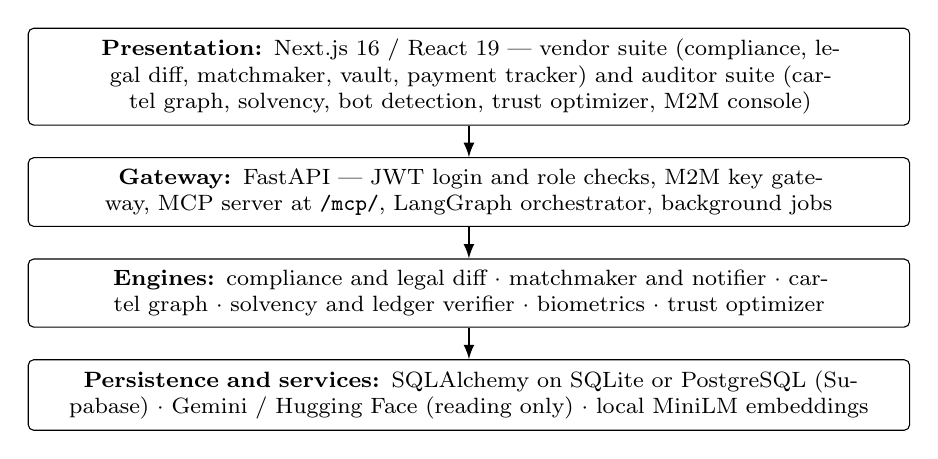
\begin{tikzpicture}[
  node distance=4mm,
  tier/.style={draw, rounded corners=2pt, text width=0.9\textwidth, align=center, inner sep=4pt, font=\footnotesize},
  arrow/.style={-latex, thick}]
\node[tier] (ui) {\textbf{Presentation:} Next.js 16 / React 19 --- vendor suite (compliance, legal diff, matchmaker, vault, payment tracker) and auditor suite (cartel graph, solvency, bot detection, trust optimizer, M2M console)};
\node[tier, below=of ui] (gw) {\textbf{Gateway:} FastAPI --- JWT login and role checks, M2M key gateway, MCP server at \texttt{/mcp/}, LangGraph orchestrator, background jobs};
\node[tier, below=of gw] (en) {\textbf{Engines:} compliance and legal diff $\cdot$ matchmaker and notifier $\cdot$ cartel graph $\cdot$ solvency and ledger verifier $\cdot$ biometrics $\cdot$ trust optimizer};
\node[tier, below=of en] (db) {\textbf{Persistence and services:} SQLAlchemy on SQLite or PostgreSQL (Supabase) $\cdot$ Gemini / Hugging Face (reading only) $\cdot$ local MiniLM embeddings};
\draw[arrow] (ui) -- (gw); \draw[arrow] (gw) -- (en); \draw[arrow] (en) -- (db);
\end{tikzpicture}
\caption{Tiers of ProcureGuard-AI.}
\label{fig:arch}
\end{figure}

The stack is Python 3.12 or later (the tests in Chapter~\ref{ch:results} ran on 3.13) with FastAPI, SQLAlchemy 2.0, LangGraph and Pydantic; PyMuPDF, Chroma and MiniLM embeddings for retrieval; NetworkX, pandas, NumPy and scikit-learn in the engines \cite{hagberg2008networkx,harris2020array,pedregosa2011scikit}; and Next.js 16.3 with React 19.2, Tailwind CSS 4 and D3 in the interface. The gateway registers 14 routers in \texttt{backend/src/main.py} (authentication, MSME profiles, legal diff, cartel, behaviour, solvency, matchmaker, notifications, tenders, documents, M2M, jobs, trust optimizer and vendor bidding) and mounts the MCP server. The web interface is a Next.js application with 14 page routes plus a landing page.

The repository also keeps the same code split into two applications, \texttt{frontend-client} (vendors, port 3000) and \texttt{frontend-admin} (auditors, port 3001). In the split vendor build the payment-tracker page is only a redirect, while the unified application has the full page; the thesis treats the unified application as the reference.

\section{Roles and Access Control}
Three roles exist: \texttt{msme} (a vendor), \texttt{government\_auditor} and \texttt{admin}. The policy sits in \texttt{backend/src/core/access.py} and is applied per router. Reviewers (auditor and admin) alone reach the cartel graph, solvency, trust optimizer, the bot-detection review queue and the MCP server. Any signed-in user can analyse tenders and run legal diff. The matchmaker, notifications and documents are limited to the owning enterprise plus reviewers, and the M2M gateway uses an API key. A test in \texttt{test\_access\_control.py} fails if any route is left unguarded, so a new endpoint cannot be added without a policy decision. The reason for such a test is that the easiest access-control mistake in a growing API is to forget a guard on a new route, and a test that enumerates the routes catches it automatically.

\section{The Tender-Analysis Pipeline}
Tender analysis is a LangGraph state graph of six nodes that share one typed state object. The graph runs in a fixed order and stops at the first failing node, returning that node's own error. Table~\ref{tab:nodes} lists the nodes; only nodes 3, 5 and 6 use a model.

\begin{table}[htbp]
\centering
\caption{Nodes of the tender-analysis graph}
\label{tab:nodes}
\small
\renewcommand{\arraystretch}{1.1}
\begin{tabularx}{\textwidth}{@{}c>{\raggedright\arraybackslash}p{3.3cm}>{\raggedright\arraybackslash}X>{\centering\arraybackslash}p{1.3cm}@{}}
\toprule
\textbf{\#} & \textbf{Node} & \textbf{Job} & \textbf{Model?} \\
\midrule
1 & \texttt{pdf\_extractor} & Text from the PDF with PyMuPDF & No \\
2 & \texttt{rag\_retriever} & Chunk, embed, keep the clauses that matter & No \\
3 & \texttt{neural\_extractor} & Clauses to typed rules with confidence and page & Reads \\
4 & \texttt{symbolic\_verifier} & Compare rules with vendor profile, compute CDS & No \\
5 & \texttt{tender\_simplifier} & Plain and regional-language summary & Explains \\
6 & \texttt{scheme\_discoverer} & Suggest support schemes for the gaps & Suggests \\
\bottomrule
\end{tabularx}
\end{table}

The graph is reachable through \texttt{POST /api/orchestrator/analyze}, or as a background job through \texttt{POST /api/jobs/tender-analyze}, which returns a job identifier that the client polls until the job is done. Section~\ref{sec:compliance} gives the method of nodes 2--4.

\subsection{Walk-through of one request}
It helps to follow a single request through the tiers. A vendor signs in and the interface stores a JWT. The vendor uploads a tender PDF and presses analyse. The gateway checks the token and the role, creates an asynchronous job record and returns its identifier. A worker runs the six nodes in order. Node 1 reads the PDF text layer; node 2 builds an in-memory index and retrieves clauses; node 3 asks a model for typed rules; node 4 compares them with the vendor's stored MSME profile and computes the scores; nodes 5 and 6 add the summary and scheme suggestions. The job record is updated with the result, and the interface, which has been polling, renders the per-rule table with its traffic-light statuses and page citations. At no point after node 3 does a model change a figure or a decision. Nodes 5 and 6 produce free text only, and the platform does not yet check that text against the typed record, so a summary could still misquote a figure; the page-cited rule table is the authoritative output.

\section{Data Model}
SQLAlchemy 2.0 maps twelve tables: \texttt{users}, \texttt{msmes}, \texttt{user\_enterprises} (which enterprises a user may act for), \texttt{tenders}, \texttt{tender\_bids} (bids placed through the vendor portal, which are the live input to the cartel and trust engines), \texttt{documents}, \texttt{async\_jobs}, \texttt{m2m\_clients}, \texttt{match\_notifications}, \texttt{behavior\_signals}, \texttt{behavior\_review\_events} and \texttt{cartel\_incident\_reviews}.

Two choices in this schema are worth explaining. Behaviour signals are stored as measurements, and each reviewer decision is a separate row in an append-only event table, so a review never changes the original score; an auditor can later see both what the detector said and what the human decided. And the user-to-enterprise link is its own table, which lets one login act for more than one enterprise. The database defaults to a local SQLite file and switches to PostgreSQL, including Supabase with row-level security, when \texttt{DATABASE\_URL} is set.

\section{Security and Reliability}
\begin{itemize}
    \item Passwords are hashed with bcrypt (12 rounds). Login tokens are HS256 JWTs valid for 24 hours. In production mode the server refuses to start without a signing secret and creates no demo accounts.
    \item The M2M gateway checks the \texttt{X-ProcureGuard-Key} header and is switched off if no key is configured. Signed requests (HMAC) are not yet verified on the server.
    \item The MCP server exposes bot-detection tools (analyse timing, list and read signals, model status), all read-only, to signed-in auditors and admins, with DNS-rebinding protection. An assistant connected through MCP cannot record or change a review.
    \item The keystroke SDK sends only timings, never characters (Section~\ref{sec:bio}). This is consistent with the data-minimisation expectations of the Digital Personal Data Protection Act 2023 \cite{dpdp2023}, but this thesis does not make a legal compliance claim.
    \item Vector indexes are built in memory per request and discarded. A background notifier scans tenders every 300 seconds by default and writes at most one notification per vendor, tender and kind, enforced by a unique constraint.
\end{itemize}

\section{Ethical and Social Considerations}
Three of the engines make statements about people or firms, and a false statement has a cost. A wrongly flagged bidder may lose business; a wrongly flagged typist may be treated as a bot. The design responds in four ways. First, nothing blocks anyone automatically: cartel, ledger and behaviour results go to a human reviewer as leads. Second, every result states its own reliability, as the keystroke score does through its low, medium and high labels. Third, the biometric input is limited to timings and no characters are recorded, which makes it much harder to recover what a person typed; timing is still treated as personal data. Fourth, because typing style differs for people who use assistive technology, the evaluation in Chapter~\ref{ch:results} reports the effect of withholding a typing style from training and does not hide it.

There is also a question of who benefits. A tool that helps small suppliers read tenders could, in principle, also help a dishonest supplier find the weakest requirement to game. The platform does not guard against that, and we do not think it can; the countermeasure is the auditor-side tooling, which is why both portals exist.

\chapter{Document Engines: Compliance, Payment and Amendments}
\label{ch:engines1}

This chapter and the next give the method of each engine, together with the constants that the code uses. File names are relative to the repository root. The three engines here work on documents, mainly for vendors: they read a tender, compute what a late payment is worth, and compare an amendment with its original.

\section{Tender Compliance}
\label{sec:compliance}

\paragraph{Retrieval.} The tender text (\texttt{agents/compliance/rag\_retriever.py}) is cut into chunks of at most 1500 characters with 200 characters of overlap, using a recursive splitter that prefers paragraph breaks. The overlap is there so that a sentence cut at a chunk boundary still appears whole in one of the two neighbours. Every chunk is embedded with the local \texttt{all-MiniLM-L6-v2} model into a 384-dimensional vector and stored in an in-memory Chroma index.

A single broad question tends to return clauses that are generally about tenders and miss the eligibility table, so five separate questions are asked (EMD, turnover, experience, MSE/startup relaxation, mandatory certificates). Each returns its four nearest chunks by cosine similarity, and the results are merged without duplicates. Retrieval is dense only; no lexical (BM25) component is used.

\paragraph{Extraction.} The merged text goes to \texttt{neural\_extractor.py}. If a Hugging Face token is set, Llama-3.1-8B-Instruct is tried first; if that fails, Gemini is tried; if that also fails, a regular-expression parser runs so that the pipeline still returns something. The model output is parsed into a Pydantic \texttt{TenderRequirements} object holding the EMD amount, required turnover, required experience, certificates, an MSME-exemption flag, and for each rule a confidence in $[0,1]$ and a source page. The temperature is 0.1, which keeps the output close to deterministic without relying on it being so.

One weakness deserves mention. When the regular-expression fallback finds nothing, it fills in default values (EMD 50{,}000, turnover 25 lakh, three years), so a fallback result must be read with care. Silently supplying thresholds also runs against the principle of Chapter~\ref{ch:design} that every figure should be traceable to a page. A cleaner design would return an explicit "not found", and this is listed under future work.

\paragraph{Verification.} From here no model is involved (\texttt{symbolic\_verifier.py}). For a numeric rule with required value $R$ and vendor value $A$, the Compliance Distance Score is
\begin{equation}
\mathrm{CDS}=\frac{A-R}{R}\times 100,
\end{equation}
which is positive when the vendor exceeds the requirement and negative when it falls short; it is 100 when there is no requirement. The score is a percentage gap, so the same number means the same thing for a rule in rupees and a rule in years.

If the tender grants an MSME relaxation and the vendor is a registered MSME, the EMD and turnover rules receive the status \texttt{EXEMPTED}. The EMD exemption follows GFR 2017 \cite{gfr2017}; the code applies the same flag to turnover, a relaxation that comes from the MSE procurement policy and that should be checked against each tender's own wording. An overall score combines the rules with fixed weights $w$ (EMD 3, turnover 2, experience 2, certificates 1):
\begin{equation}
\mathrm{OCD}=\frac{\sum_i w_i\,n_i}{\sum_i w_i},\qquad
n_i=\begin{cases}100 & \text{pass or exempted}\\ \max(0,\,100+\mathrm{CDS}_i) & \text{fail.}\end{cases}
\end{equation}
Each rule also carries a traffic-light status and a human-readable reason, so the result can be traced from the report back to the clause and page.

\paragraph{Worked example.} Take a tender that requires a turnover of Rs~25 lakh and three years of experience, grants the MSE relaxation (which the code applies to EMD and turnover together), and asks for one certificate. A registered micro enterprise has a turnover of Rs~40 lakh, two years of experience and the certificate. The turnover rule gives $\mathrm{CDS}=(40-25)/25\times100=+60$, which is still reported, but its status is exempted. The experience rule gives $\mathrm{CDS}=(2-3)/3\times100\approx-33.3$ and fails, so its contribution is $n=100-33.3=66.7$. The EMD rule is also exempted and the certificate passes, so all three contribute 100. Then
\begin{equation}
\mathrm{OCD}=\frac{3(100)+2(100)+2(66.7)+1(100)}{3+2+2+1}=\frac{733.3}{8}\approx 91.7.
\end{equation}
The report would show one amber row (experience, 33\% short) and three green rows, and the vendor sees exactly which clause to address. The failure does not disappear into an average, because each rule keeps its own status next to the overall score. Two caveats apply. An exempted rule counts as 100, so an exempt vendor receives the full weight of those rules for free; dropping exempted rules from both sums would be a fairer score. And OCD is a gap measure, not a verdict: a failed mandatory rule is usually a disqualification in practice, so the per-rule status, and not the average, is what the vendor should act on. The exemption is also decided by a single registered-MSME flag, whereas the GFR relaxation itself covers micro and small enterprises only, so a medium enterprise would be wrongly exempted.

\paragraph{Failure modes.} The engine can go wrong in three places. The retriever may miss the clause, in which case the extractor has nothing to read. The extractor may read a figure wrongly, for instance taking the turnover of the previous year for the required turnover. And the vendor profile may be out of date. The first two are the reasons that every rule carries a page number and a confidence: the vendor can open the page and check. The third is outside the engine's control.

\section{Statutory Payment Recovery}
\label{sec:payment}
Section 15 of the MSMED Act sets the payment period at 45 days, and Section 16 makes the buyer liable for compound interest with monthly rests at three times the RBI bank rate \cite{msmedact2006}. The module (\texttt{payment\_tracker.py}) uses a bank rate of 6.5\%, so $r=19.5\%$ a year. With $D$ the days from invoice to payment, the overdue days are $D-45$ if that is positive, and the number of monthly rests is $m=\lceil (D-45)/30\rceil$. The amount owed is
\begin{equation}
A=P\left(1+\frac{r}{12}\right)^{m},\qquad I=A-P.
\end{equation}

\paragraph{Worked examples.} An invoice of Rs~5{,}00{,}000 paid 90 days after the invoice date is 45 days overdue, so $m=2$ and
\begin{equation}
I=500000\left[(1.01625)^2-1\right]\approx \text{Rs}~16{,}382.
\end{equation}
A smaller invoice of Rs~2{,}00{,}000 paid after 120 days is 75 days overdue, so $m=\lceil 75/30\rceil=3$ and $I=200000\,[(1.01625)^3-1]\approx\text{Rs}~9{,}909$. The monthly rate is $19.5/12=1.625\%$ in both cases.

\paragraph{Assumptions.} Rounding part-months up slightly overstates the interest, and measuring from the invoice date rather than from acceptance is a known simplification. The bank rate is a constant in the code and would need to be updated when the RBI changes it, so the figures above are illustrative at a 6.5\% rate; we did not check that value against the rate currently notified by the RBI, and it is not a statement of the current statutory rate. The invoice itself is read by a vision model, but only the extracted principal and dates enter the formula, and the vendor confirms them before a draft demand notice is produced. A wrong date therefore costs the vendor a correction, not a wrong legal claim.

\section{Corrigendum Differ}
\label{sec:differ}
Both documents are split into clauses and embedded with the same MiniLM model. For each original clause the most similar amended clause is found by cosine similarity, and the pair is flagged when that best similarity is below 0.75 (\texttt{semantic\_differ.py}). Comparing by embedding and not by character difference means that a reworded but equivalent clause is not flagged. The method has two weaknesses that Chapter~\ref{ch:results} does not evaluate systematically. Sentence embeddings change very little when only a number is altered. In a quick check on hand-written clause pairs (not a systematic evaluation), raising a turnover requirement from Rs~2 crore to Rs~5 crore gave a cosine similarity of 0.96, raising an EMD tenfold gave 0.95, and moving a deadline gave 0.95; even a pair that raised the experience requirement from three to ten years and added a new condition scored 0.81. All of these stay above 0.75 and would go unflagged. The clause pairs are not part of the repository's experiment scripts, so these four values are indicative only and cannot be reproduced from this thesis. And because the search runs from the original clauses, a wholly new clause has nothing to match against. A numeric and date comparison alongside the embedding, and a search in both directions, are the obvious remedies and are listed under future work.

A model then labels each flagged pair \texttt{RESTRICTIVE}, \texttt{PERMISSIVE} or \texttt{NEUTRAL}; this is the only model step, and because the label sets the base score it does influence the verdict. The rule is therefore that the model reads and labels while code computes, not that the model has no effect. The rest is arithmetic (\texttt{corruption\_risk\_scorer.py}). Each restrictive clause adds 0.3 and each neutral clause 0.1; the sum is capped at 1. A time multiplier $\tau$ is 3.0 if the amendment is at most 2 days before the deadline, 1.5 if at most 7 days, and 1.0 otherwise. The manipulation probability is
\begin{equation}
p=\min\bigl(0.99,\ \tau\cdot\min(1,\textstyle\sum_k b_k)\bigr),
\end{equation}
where $b_k$ is the base score of flagged clause $k$. A result is \texttt{CRITICAL} for $p\ge 0.75$, \texttt{SUSPICIOUS} for $p\ge 0.40$ and \texttt{SAFE} otherwise. The multiplier is a step function.

\paragraph{Worked example.} Suppose an amendment changes one clause and the model labels it restrictive, so $\sum_k b_k=0.3$. The risk depends on timing alone:
\begin{center}
\small
\begin{tabular}{@{}lccl@{}}
\toprule
\textbf{Amendment issued} & $\tau$ & $p$ & \textbf{Verdict} \\
\midrule
10 days before deadline & 1.0 & 0.30 & \texttt{SAFE} \\
6 days before deadline & 1.5 & 0.45 & \texttt{SUSPICIOUS} \\
1 day before deadline & 3.0 & 0.90 & \texttt{CRITICAL} \\
\bottomrule
\end{tabular}
\end{center}
The same clause change is treated as harmless early and as critical at the last moment, which is the behaviour intended: a restrictive change that leaves bidders time to respond is ordinary, and one that does not is a warning sign. The step function makes the thresholds easy to explain to a reviewer, at the cost of a jump at 2 and 7 days.

\chapter{Auditor Engines: Collusion, Ledger, Behaviour and Trust}
\label{ch:engines2}

The four engines in this chapter serve auditors. They work on relations between bidders, on the internal consistency of financial documents, on timing signals from the bid form, and on the ranking of bidders. Each of them produces a lead for a human reviewer, not a verdict.

\section{Cartel Graph}
\label{sec:cartel}
\paragraph{Structure.} The graph (\texttt{engines/cartel\_graph/graph.py}) is bipartite: one side holds bidders, the other holds shared attributes of four kinds (directors, IP addresses, bank routing codes, and declared assets or certificates). Blank or missing values never become nodes, so two bidders with nothing recorded cannot match each other. This is a small rule but it matters, because missing data is common and treating "empty" as a shared value would link unrelated firms.

\paragraph{Evidence weight.} An attribute node with degree $d\ge 2$ becomes a piece of evidence with weight
\begin{equation}
w(d)=\min\!\left(1,\ \frac{1}{\ln(1+d)}\right).
\end{equation}
This is the inverse-logarithm weight used by Adamic and Adar for shared neighbours in social networks \cite{adamic2003friends}: the more bidders share an attribute, the less it says about any two of them. Table~\ref{tab:weights} gives some values.

\begin{table}[htbp]
\centering
\caption{Evidence weight $w(d)$ of a shared attribute held by $d$ bidders}
\label{tab:weights}
\small
\begin{tabular}{@{}lcccccc@{}}
\toprule
$d$ & 2 & 3 & 4 & 5 & 6 & 10 \\
\midrule
$w(d)$ & 0.910 & 0.721 & 0.621 & 0.558 & 0.514 & 0.417 \\
\bottomrule
\end{tabular}
\end{table}

The decay is slow, so the discount is mild and not strong. For stronger protection, an IP or bank code shared by more than five bidders (the default cap, \texttt{AEGIS\_PUBLIC\_DEGREE\_CAP}) is treated as public infrastructure and can never flag anyone on its own. A shared director is not subject to the cap, since a real person sitting on many boards is exactly what an auditor wants to see. Bidders that appear together in a declared joint-venture group are exempt from each other.

\paragraph{Pair flags.} A pair of bidders is flagged when they share at least one attribute that is not public infrastructure and is not covered by a declared joint venture; there is no separate score threshold. The weight $w(d)$ does not decide the flag. It scales how much each shared attribute adds to a bidder's anomaly score below.

\paragraph{Rings.} Flagged pairs are merged into rings by taking connected components of a bidder--evidence graph, so five colluding firms appear as one ring and not as ten pairs. For an auditor this changes the question from "which pairs look related?" to "which groups look coordinated?", which is closer to how a cartel is actually described in an enquiry. Because rings are connected components, a chain of weak links (A and B share an IP, B and C share a bank code) can merge unrelated bidders into one ring, and the auditor should read a ring as a lead and not as a finding.

\paragraph{Anomaly score.} Each bidder also receives an anomaly score (\texttt{scoring.py}). Let $\bar a$, $\bar o$ and $\bar n$ be the weighted counts of shared assets, shared owners and shared network attributes, divided by the bidder's declared assets, owners and two respectively. With clamping to $[0,1]$,
\begin{equation}
A_i=\mathrm{clamp}\bigl(0.45\,S_a+0.35\,S_o+0.20\,S_c-0.30\,\rho_i\bigr),
\end{equation}
where $S_a=\mathrm{clamp}(1.6\bar a)$, $S_o=\mathrm{clamp}(1.8\bar o)$, $S_c=\mathrm{clamp}(0.75\bar n+0.75\bar a)$ and $\rho_i=\min(1,0.8\cdot\text{partners sharing assets}/\text{declared assets})$.

The sign of the $\rho_i$ term is worth noting: the code subtracts it, although its comment says it should raise suspicion. Because shared assets already enter $S_a$ and $S_c$, the subtraction acts as a calibration term. We report the behaviour as implemented and list the question under future work. Read literally, it means that a bidder whose partners share its assets receives a lower score than it otherwise would, which is the opposite of what a collusion detector should do, so the term needs either a code fix or a stronger justification.

\paragraph{Cost.} Building the graph is linear in the number of bidder--attribute edges. The pair search compares every pair of bidders, so it is quadratic in the number of bidders in a pool. For the pools of a dozen or a few dozen bidders that a single tender attracts this is negligible, but it would need an index over attribute nodes before it could be run across a whole portal.

\section{Ledger-Constrained Bank-Statement Verification}
\label{sec:ledger}
The verifier (\texttt{engines/solvency/ledger\_verifier.py}) treats a statement as a ledger and applies five constraints, with a tolerance $\epsilon=0.05$ rupees. The first is the strongest, because it is an identity and not a statistical test.

\paragraph{1. Row recurrence and OCR repair.} For each row, $|B_t-(B_{t-1}+C_t-D_t)|\le\epsilon$. If a row fails, the verifier generates candidates by replacing one digit of the integer part of the balance, the credit or the debit with a visually confusable digit (1/7, 3/8, 8/0, 5/6, and the corresponding letter confusions), and searches the combinations. If some combination satisfies the recurrence the row is marked \texttt{CORRECTED\_OCR\_ERROR} and the repaired balance is carried forward; otherwise it is an \texttt{UNEXPLAINABLE\_RESIDUAL} and raises a critical flag.

\emph{Illustration.} Suppose a row opens at Rs~95{,}000 with a credit of Rs~23{,}000, so the balance should be Rs~1{,}18{,}000. If the scan reads 7{,}18{,}000, the recurrence fails; changing the 7 to a 1 restores it, so the row is repaired and the correct balance is carried forward. If the document instead shows Rs~1{,}68{,}000, as it would after a Rs~50{,}000 insertion, no single confusable swap in the balance, credit or debit satisfies the recurrence, and the row is flagged as unexplained.

A forgery could in principle coincide with a confusion swap and be mistaken for scanning noise. The experiment in Section~\ref{sec:res_ledger} measures how often that happens.

\paragraph{2. Page continuity.} The opening balance of page $p+1$ must equal the closing balance of page $p$, which exposes deleted or spliced pages.

\paragraph{3. Window dressing.} A robust $Z$-score compares the mean balance of the last 30 days with the earlier history:
\begin{equation}
Z=\frac{\overline{B}_{30}-\mathrm{median}(B_{\text{prior}})}{1.4826\cdot\mathrm{MAD}(B_{\text{prior}})},
\end{equation}
flagged when $Z\ge 3$. The constant 1.4826 makes the MAD comparable to a standard deviation for normally distributed data, and the median and MAD resist single outliers \cite{rousseeuw1993alternatives}.

\paragraph{4. Round trips.} A credit of at least twice the median credit is matched to a debit within the next 7 days whose amount differs by at most 2\% and whose narration shares more than one token with the credit. This catches the pattern in which money enters shortly before submission and leaves again shortly after.

\paragraph{5. Benford check.} With at least 30 amounts, the largest gap between the observed first-digit proportions and $\log_{10}(1+1/d)$ \cite{benford1938law,nigrini2012benford} is computed, and a low-severity flag is raised if it exceeds 0.25. This is a maximum-deviation statistic, not a full Kolmogorov--Smirnov test, and it only signals suspicion. The value 0.25 is a default that was not tuned or validated here; it is lax, so only strongly non-Benford amounts would be flagged.

The solvency figure reported to auditors is a time-weighted average balance, so a one-day spike has little effect on it.

\section{Keystroke Bot Detection}
\label{sec:bio}
\paragraph{Capture and features.} The browser SDK records only key-down and key-up times. Hold time is $H_k=t^{\text{up}}_k-t^{\text{down}}_k$ and flight time is $F_k=t^{\text{down}}_k-t^{\text{up}}_{k-1}$. Flights are clipped at 2000 ms and holds at 1000 ms so that a pause to read the form cannot dominate, and the first flight (the delay before typing starts) is discarded.

The features (the feature module of the biometrics engine) fall into four groups, shown in Table~\ref{tab:feat}. All are defined so that they do not grow with the number of keystrokes, but their estimates are noisier for short sessions, which is why every score carries a reliability label.

\begin{table}[htbp]
\centering
\caption{Feature groups used by the keystroke detector}
\label{tab:feat}
\small
\renewcommand{\arraystretch}{1.1}
\begin{tabularx}{\textwidth}{@{}>{\raggedright\arraybackslash}p{3.6cm}>{\raggedright\arraybackslash}X@{}}
\toprule
\textbf{Group} & \textbf{Content} \\
\midrule
Location and spread & Means, spreads and percentiles of log hold and log flight times \\
Shape & Skewness and kurtosis of the log timings \\
Rhythm & Lag-1 autocorrelation of the flight series \\
Interval mix & Share of short, long and pause intervals \\
\bottomrule
\end{tabularx}
\end{table}

\paragraph{Model.} The log features are modelled by a Gaussian mixture \cite{bishop2006prml}
\begin{equation}
p(\mathbf{x})=\sum_{j=1}^{J}\pi_j\,\mathcal{N}(\mathbf{x}\mid\mathbf{m}_j,\boldsymbol\Sigma_j),
\end{equation}
fitted by expectation--maximisation \cite{dempster1977maximum} on genuine human sessions only, with $J=2$ components for the full mode (hold and flight) and $J=4$ for the flight-only fallback; $\mathbf{m}_j$ and $\boldsymbol\Sigma_j$ are the mean and covariance of component $j$. A mixture is used because human typists are not one population: a fast typist and a slow one form two clusters, and a single Gaussian would call the space between them normal. These sizes were selected on a separate development dataset (seed 7) as the simplest candidate within 1\% of the best macro detection rate at a human false-alarm rate near 5\%.

The negative log-likelihood is mapped to a 0--100 risk score using a threshold calibrated per session-length band on a held-out human split, so that 50 is meant to be the 95th percentile of humans of similar length and 75 the 99th (Section~\ref{sec:res_bio_len} shows that the realised false-alarm rate still varies with length). A session is moderate risk from 50 and high risk from 75. A reliability label accompanies every score: low below 30 keystrokes, medium from 30 to 99, high from 100. Models are exported as JSON and scored with NumPy alone \cite{harris2020array}, so no training library is needed at the point of use.

\paragraph{Use.} The score is advisory. Sessions that need review enter a pending queue, each reviewer decision is stored as its own event, and nothing ever blocks a bid automatically, because people who use assistive technology type differently from the training population.

\section{Bayesian Trust Optimizer}
\label{sec:trust}
For a tender with reference price $B_{\text{ref}}$ (the independent estimate), five agents score each bidder (\texttt{engines/trust\_optimizer}).
\begin{align}
P_i&=\delta\frac{B_{\min}}{B_i}+(1-\delta)\frac{B_{\text{ref}}}{B_i},\quad \delta=0.5,\\
\mathrm{Perf}_i&=\frac{\sum_k v_ks_{ik}+\alpha}{\sum_k v_k(s_{ik}+f_{ik})+\alpha+\beta},\quad \alpha=\beta=1,\\
L_i&=\exp\!\Bigl(-\bigl[\textstyle\sum_c n^{\text{ver}}_{ic}w_c+\gamma D_i\bigr]\Bigr),\quad \gamma=2,
\end{align}
where $n^{\text{ver}}_{ic}$ is the number of verified cases of category $c$ for bidder $i$ and $w_c$ is the weight of that category.

\paragraph{Price.} Bids more than 40\% from $B_{\text{ref}}$ are excluded when finding $B_{\min}$, so shell bids cannot move the price scale. Bids that far below $B_{\text{ref}}$ therefore cannot lower the scale, and the eligibility gate is intended to stop them from winning on price alone (the simulation of Chapter~\ref{ch:results} shows one such case, not a guarantee). The price score itself is a ratio, so a very low bid that passes the gate still scores higher; capping $P_i$ at 1 would remove this and is listed under future work.

\paragraph{Performance.} The performance score is a Beta-style estimate in the manner of the beta reputation system \cite{josang2002beta}, in which $s_{ik}$ and $f_{ik}$ are the successful and failed projects of bidder $i$ with client $k$. Each is weighted by a verification weight $v_k$, so that mutual-reference rings count for less. The prior $\alpha=\beta=1$ pulls a bidder with no history towards 0.5 and not towards either extreme.

\paragraph{Legal.} In the legal score, $D_i$ counts audited cases above self-declared cases in each category, so under-declaring litigation is penalised.

\paragraph{Financial and technical.} The financial score scales the product of liquidity, credit rating and profitability between a floor and a ceiling, after an eligibility gate on registration age (two years) and turnover. The technical score is a Cobb--Douglas product \cite{cobb1928theory} of equipment, staff, technology and experience ratios, multiplied by a uniqueness factor $u_i=1-|\text{assets}_i\cap\text{assets}_{-i}|/|\text{assets}_i|$ that reduces the score when equipment is shared with other bidders. The price score is not bounded by 1; it reached 2.5 in the simulation.

\paragraph{Fusion and selection.} A fused trust value $T_i=\sum_jC_{ij}\eta_jT_{ij}/\sum_jC_{ij}\eta_j$ combines the agent scores using confidences $C$ (project and case counts) and multipliers $\eta_j\in[0.85,1.15]$ drawn from a generator seeded by the tender identifier, so weights are reproducible for a given tender. Because the identifier is public, this is variation and not secrecy: it stops one fixed set of weights from being tuned against, but anyone with the code can recompute it. Selection removes bidders failing the gate or the minimum thresholds (each jittered by up to $\pm0.02$ per tender, which like the weights is recomputable from the public tender identifier and so adds variation, not security), then ranks the rest by
\begin{equation}
Z_i=\sum_k w_kS_{ik}-\mu A_i,\qquad \mu=0.3,
\end{equation}
where $S_{ik}$ is the score of bidder $i$ from agent $k$, $w_k$ is the weight of that agent, and $A_i=(S_a+O_i+S_c)/3$ averages shared-asset share, ownership overlap and score clustering (another bidder within Euclidean distance 0.05), or is replaced by the cartel engine's score for real bids. If the top two values differ by less than 0.02 and either bidder has $A\ge0.10$, the award is held for manual review. After the project, trust is updated as $T^{\text{new}}=0.8\,T^{\text{old}}+0.2\,o$ for outcome $o\in[0,1]$, so one project moves the value by at most 20\% of the gap.

\chapter{Results and Discussion}
\label{ch:results}

Every number in this chapter comes from a file or a command in the repository, or from one of the scripts {\small\path{thesis/experiments/rq2_experiments.py}} and {\small\path{thesis_amrita/experiments/cap_sweep.py}}. All data are synthetic. Where a result is weak we say so in the same paragraph that reports it.

\section{Evaluation Setup and Metrics}
Since no real procurement or typing data was available, each engine is evaluated on data produced by a generator with a fixed random seed. This makes every experiment repeatable, but it also means that the results describe the engine under the generator's assumptions. The measures used are the following.

\begin{itemize}
    \item \textbf{False-alarm rate}: the share of genuine cases that are flagged. For the keystroke detector this is the share of human sessions with risk at or above 50.
    \item \textbf{Detection rate}: the share of attack cases that are flagged. The macro detection rate is the unweighted mean over the three core attack types, so that no single attack dominates.
    \item \textbf{ROC-AUC}: the probability that a randomly chosen attack session receives a higher risk score than a randomly chosen human session \cite{fawcett2006roc}. It summarises ranking quality independent of any threshold.
    \item \textbf{Wilson interval}: the 95\% confidence interval for a proportion, used for the detection and false-alarm rates because it behaves sensibly near 0 and 1 \cite{wilson1927probable}.
\end{itemize}

\section{Test Suites}
We ran the suites on the final repository (Windows, Python 3.13). Table~\ref{tab:tests} gives the outcome.

\begin{table}[htbp]
\centering
\caption{Automated test results on the final repository}
\label{tab:tests}
\small
\begin{tabularx}{\textwidth}{@{}>{\raggedright\arraybackslash}p{4.4cm}>{\raggedright\arraybackslash}X@{}}
\toprule
\textbf{Suite} & \textbf{Result} \\
\midrule
Cartel, solvency, trust optimizer & 21 passed \\
Backend gateway & 162 passed, 5 failed, 4 skipped \\
Biometrics engine & 219 passed (the browser test and two modules needing \texttt{pytest-asyncio} were excluded from this run) \\
\bottomrule
\end{tabularx}
\end{table}

The five backend failures are one test in \texttt{test\_rule\_retrieval.py} and four in \texttt{test\_vendor\_portal.py}. The first expects an error when both language-model providers fail, but the extractor now falls back to the regular-expression parser, so the test is out of date. In the other four, which concern the shipped bidder pool and IP fields, the cause was not diagnosed; they may depend on state in the local database. We report them as failures and do not hide them.

\section{Keystroke Detector (RQ3)}
\label{sec:res_bio_len}
The protocol is in \texttt{engines/biometrics/reports/evaluation\_report.md} \cite{bioreport}. A generator with seed 42 produced 39{,}000 sessions of 10--300 keystrokes, with lengths drawn log-uniformly so that short and long sessions are both common. Genuine humans (typical, fast and slow typists) were split 60/25/15 into training, calibration and test by session; bots appear only in evaluation. The four bot classes differ in how closely they imitate a person. A regular script types at a perfectly even rhythm. Burst injection sends small chunks of characters separated by pauses. The adaptive bot varies its timing to look human, and its hold times are the main thing that betrays it (see the flight-only result below). The mimic bot is a stress test that copies the mean, spread and pause rate of human typing. Table~\ref{tab:bio} shows the full model.

\begin{table}[htbp]
\centering
\caption{Full-model detection at risk $\ge 50$ (95\% Wilson intervals)}
\label{tab:bio}
\small
\begin{tabular}{@{}lrl@{}}
\toprule
\textbf{Class} & \textbf{Sessions} & \textbf{Flagged} \\
\midrule
Genuine humans (all three styles) & 2700 & 4.6\% (3.8--5.4) \\
Regular script & 6000 & 100.0\% (99.9--100) \\
Burst injection & 6000 & 100.0\% (99.9--100) \\
Adaptive bot & 6000 & 54.6\% (53.4--55.9) \\
Mimic bot (stress test) & 3000 & 44.7\% (42.9--46.5) \\
\midrule
Macro detection (three core attacks) & & 84.9\% \\
ROC-AUC (core attacks vs.\ humans) & & 0.958 (0.955--0.960) \\
\bottomrule
\end{tabular}
\end{table}

Detection of the adaptive bot depends strongly on session length (Figure~\ref{fig:biolen}): 13\% for 10--19 keystrokes, 40\% for 30--49, 92\% for 100--199 and 98\% for 200--300. The figure shows four of the six length bands; the other two, 20--29 and 50--99 keystrokes, give 24\% and 68\%. A short session simply carries too little evidence, and it also raises false alarms on humans: 7.5\% of genuine sessions of 10--19 keystrokes are flagged, against 2.4\% at 200--300, so the length-band thresholds of Section~\ref{sec:bio} do not equalise the false-alarm rate across lengths. In flight-only mode the human false-alarm rate is unchanged at 4.6\%, but macro detection drops to 67.3\% and the adaptive bot is almost invisible (1.9\%), because without hold times it cannot be told apart from a human.

\begin{figure}[htbp]
\centering
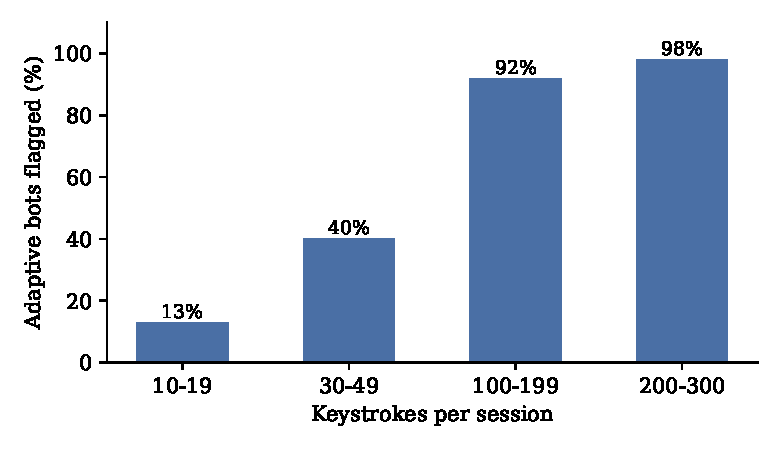
\includegraphics[width=0.72\textwidth]{fig_bio_length.pdf}
\caption{Share of adaptive-bot sessions flagged at risk $\ge 50$, by session length (full model).}
\label{fig:biolen}
\end{figure}

Table~\ref{tab:cmp} compares the shipped mixture with the Isolation Forest of the first design, both calibrated to the same false-alarm budget on the same data.

\begin{table}[htbp]
\centering
\caption{Detector comparison, full mode, same data and false-alarm budget}
\label{tab:cmp}
\small
\begin{tabular}{@{}lrrrr@{}}
\toprule
\textbf{Detector} & \textbf{Adaptive} & \textbf{Mimic} & \textbf{Macro} & \textbf{AUC} \\
\midrule
Gaussian mixture (shipped) & 54.6\% & 44.7\% & 84.9\% & 0.958 \\
Isolation Forest, PCA-whitened & 47.3\% & 19.4\% & 82.4\% & 0.951 \\
Isolation Forest, standardised only & 2.4\% & 4.0\% & 67.5\% & 0.897 \\
\bottomrule
\end{tabular}
\end{table}

The comparison shows that preprocessing mattered as much as the choice of detector. The same Isolation Forest that nearly misses the adaptive bot (2.4\%) when features are only standardised reaches 47.3\% after PCA whitening, close to the mixture. The mixture was kept because it was ahead on every column and because it can be exported as plain parameters.

\paragraph{Limits.} When bots are rare a flag is weak evidence: at a 1\% share of automated sessions the precision of a risk-50 flag is 15.8\%, which is why the output is advisory. A held-out typing style is the larger risk: when one human style was withheld from training and calibration, 51--81\% of its sessions were flagged. The model treats the training population as normal, and real deployment would require retraining on real bidders. The scoring latency measured on an AMD64 machine under Windows is a p95 of 0.54 ms in process and 3.4 ms through an in-process ASGI call, within the 15 ms target but excluding network time.

These results support RQ3 for synthetic sessions only. They show that timing separates crude automation from human typing, and that it is much weaker against bots that imitate human timing.

\section{Ledger Repair (RQ2)}
\label{sec:res_ledger}
We generated 500 statements of 40 rows for each of three conditions, with integer rupee amounts and a valid recurrence. In the OCR condition one balance digit was replaced by its confusable partner. In the tamper condition one balance was inflated by Rs~5{,}000--2{,}00{,}000. The strict check applies the recurrence with no repair; the lattice check is the engine's row verifier. Table~\ref{tab:ledger} shows the number of statements flagged.

\begin{table}[htbp]
\centering
\caption{Statements flagged out of 500 per condition}
\label{tab:ledger}
\small
\begin{tabular}{@{}lrr@{}}
\toprule
\textbf{Condition} & \textbf{Strict recurrence} & \textbf{With OCR lattice} \\
\midrule
Clean & 0 & 0 \\
Scanning noise (benign) & 500 & 17 \\
Tampered balance & 500 & 500 \\
\bottomrule
\end{tabular}
\end{table}

The lattice cleared 483 of 500 noisy statements (96.6\%) and missed none of the 500 tampered ones. Without it, a strict check would send every scanned statement to a human, which is the practical argument for the repair step.

The 17 remaining noise cases were not traced individually; the cause was traced on a separate sample (36 of 1000): the search accepts the first combination that satisfies the recurrence, and sometimes that combination changes the credit or debit and not the corrupted balance. The corrupted balance is then carried forward and the next row fails, so the statement is still flagged, but at the wrong row. This is a weakness in how the repair is attributed. A tampering that happens to equal a confusion swap could be explained away in the same manner, although none of the 500 random inflations was. This result is also easier than it looks: the inflations were drawn at random, so only a small share of them could coincide with a single-digit confusion swap (a 1 changed to a 7 in the thousands place, for example, adds exactly Rs~6{,}000), and 500 of 500 is close to the expected outcome. A forger who edits with confusable digits was not tested, and that is the case in which the repair step could excuse a real forgery. The simulation is also simple (one error per statement, uniform amounts), so the real rate will differ.

\section{Cartel Graph (RQ2)}
Each of 300 synthetic pools has exactly 12 bidders (66 pairs) with unique directors and assets, an IP chosen from three shared addresses and a bank code from four shared codes, as when firms use a common provider and branches. In 120 pools three random bidders also share one director (a planted ring). A naive method flags every pair sharing any attribute; the engine's \texttt{build\_cartel\_summary} is compared with it. A pool with a planted ring has $66-3=63$ honest pairs and one without has 66, so the total is $120\times63+180\times66=19{,}440$ honest pairs.

\begin{table}[htbp]
\centering
\caption{Cartel experiment at the default cap: 300 pools, 19{,}440 honest bidder pairs}
\label{tab:cartel}
\small
\begin{tabular}{@{}lr@{}}
\toprule
\textbf{Measure} & \textbf{Value} \\
\midrule
Honest pairs flagged, naive method & 9{,}655 \\
Honest pairs flagged, engine & 6{,}771 (29.9\% fewer) \\
Planted rings fully recovered & 120 of 120 \\
Mean anomaly score, ring members & 0.320 \\
Mean anomaly score, other bidders & 0.093 \\
\bottomrule
\end{tabular}
\end{table}

The engine never missed a ring, and ring members score about three times higher than other bidders. The reduction in false pairs is modest at the default cap. With 12 bidders over 3 addresses each address is shared by four firms on average, so the cap, which applies only to groups of more than five, affects only the larger random groups and removes only part of the false pairs. The sweep below shows how much of the result depends on that one parameter.

\subsection{Sensitivity to the public-infrastructure cap}
To see how much of the result is a consequence of the cap, we repeated the experiment with the cap set to 2, 3, 4, 5, 6 and 8, using the environment variable \texttt{AEGIS\_PUBLIC\_DEGREE\_CAP} and the same pools. The results are in Table~\ref{tab:cap} and Figure~\ref{fig:cap}.

\begin{table}[htbp]
\centering
\caption{Honest pairs flagged by the engine for different caps (naive method: 9{,}655)}
\label{tab:cap}
\small
\begin{tabular}{@{}lrrr@{}}
\toprule
\textbf{Cap} & \textbf{Honest pairs flagged} & \textbf{Reduction vs.\ naive} & \textbf{Rings recovered} \\
\midrule
2 & 375 & 96.1\% & 120 of 120 \\
3 & 1{,}877 & 80.6\% & 120 of 120 \\
4 & 4{,}199 & 56.5\% & 120 of 120 \\
5 (default) & 6{,}771 & 29.9\% & 120 of 120 \\
6 & 8{,}356 & 13.5\% & 120 of 120 \\
8 & 9{,}532 & 1.3\% & 120 of 120 \\
\bottomrule
\end{tabular}
\end{table}

\begin{figure}[htbp]
\centering
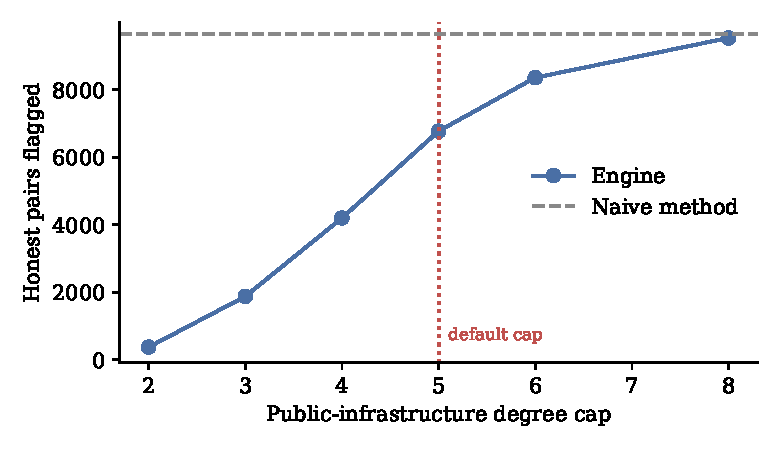
\includegraphics[width=0.72\textwidth]{fig_cap_sweep.pdf}
\caption{False pairs flagged by the engine as the public-infrastructure cap varies.}
\label{fig:cap}
\end{figure}

The 29.9\% reduction is therefore a property of the cap, not of the engine. The degree-discounted weight $w(d)$ does not enter the pair flag at all, so it plays no part in this reduction. A cap of 3 removes about four fifths of the false pairs here, and a cap of 8 removes almost none. Ring recovery stays perfect at every setting, but this must not be over-read. The planted rings are linked by a shared director, and directors are never capped, so lowering the cap cannot hurt recall in this experiment by construction. In real data a ring that shared only an IP address or a bank branch would be hidden by a low cap. The experiment cannot measure that cost, and the right cap has to be chosen on real bidder data, with the trade-off between nuisance flags and missed rings made explicitly. The pair list also still needs the anomaly score to be useful. Even at the default cap the engine flags 6{,}771 of 19{,}440 honest pairs (34.8\%), and the 29.9\% figure is measured against a deliberately naive baseline, so the experiment does not show a useful false-alarm rate on real bidders.

\section{Trust Optimizer Simulation}
The bundled simulation (\texttt{run\_simulation.py}, seed 42) ranks 20 bidders for one tender. The two colluders have anomaly 0.833 and are both excluded, but not by the collusion penalty: both fail the technical minimum (a technical score of 0.2324 against a threshold of about 0.3), and the penalty $\mu A_i$ would only have lowered their composite score by about 0.25. In this run the anomaly score therefore did not decide the outcome. Only 7 of the 20 bidders pass the gates, and the winner, B020, has a fused trust of 0.8376 and a price score of 1.17. A bidder with a very low price but the lowest financial score is stopped by the eligibility gate, and a bidder that under-declared litigation receives a legal score of 0.0012. The winner's trust becomes 0.8700 after a successful project and 0.6700 after a failed one. These are constructed cases, not an accuracy measurement. They show the eligibility gate, the legal penalty and the trust update acting on cases built to trigger them. They do not show the collusion penalty $\mu A_i$ changing an outcome, so that safeguard remains untested in this thesis.

\section{Tender Pipeline (RQ1)}
The project README reports an end-to-end run on a real GeM tender whose extracted EMD, turnover (Rs~27 lakh), experience (three years) and MSE exemption match the document. We did not repeat it for this thesis, since it needs a model key, so it is reported as anecdotal. The unit tests check CDS values, exemption handling and the orchestrator graph. No experiment here measures how often the extractor is wrong or how often the symbolic layer catches the error, so RQ1 is supported by design and tests but not by an error-rate study.

\section{Discussion and Threats to Validity}
The biometrics engine has the most extensive evaluation here (the largest sample, confidence intervals and a baseline comparison), but all of it is synthetic, so none of the engines is validated on real data. The main threats are:
\begin{itemize}
    \item \textbf{Synthetic data.} Detector and experiment results depend on the generators that the project authors wrote, and the mixture size was chosen on a development set built from the same generator. They show behaviour under stated assumptions, not field accuracy.
    \item \textbf{Own experiments.} We wrote the ledger and cartel experiments to test the safeguards, so they may favour the design. The cap sweep partly guards against this, since it shows a setting where the safeguard looks weak.
    \item \textbf{Untested paths.} The scanned-PDF OCR route and live Gemini extraction were not exercised here, and five tests fail.
    \item \textbf{Single seeds.} The experiments use one seed each. The Wilson intervals describe sampling error within a seed, not variation between generators.
\end{itemize}

Taken together, the results say something consistent. The safeguards work in the direction intended, although their cost (for example the wrongly cleared forgeries or missed rings they may cause on real data) was not measured, and each one has a parameter or an assumption that decides how much it helps: the cap in the cartel graph, the single-error assumption in the ledger repair, and the session length for the keystroke detector. A reader who wants to rely on any of these engines should treat the parameter as the thing to calibrate first.

\chapter{Conclusion and Future Work}
\label{ch:conclusion}

\section{Summary}
ProcureGuard-AI is a working platform in which language models read and explain while deterministic code decides. It offers vendors a tender eligibility check with page citations, a late-payment interest calculator, a corrigendum differ and a joint-venture matchmaker. It offers auditors a cartel graph, a bank-statement verifier, a keystroke bot detector and a collusion-resistant trust optimizer. All of these sit behind one role-controlled API, and each engine can be run and tested separately.

The central design decision was where to draw the line between the model and the code. Drawing it at the typed record, so that the model's output is parsed into a schema and nothing after that point is generated, gave a system whose decisions can be replayed and whose figures can be checked against a page. It also meant that a large part of the work was ordinary engineering: statutory formulas, graph weights, accounting identities and calibrated thresholds.

\section{Answers to the Research Questions}
\begin{enumerate}
    \item \textbf{RQ1.} The design makes each decision repeatable and traceable, and unit tests confirm the scoring and exemption logic. The thesis did not measure extractor error rates, so the benefit against hallucination is argued from the design and not shown by an experiment.
    \item \textbf{RQ2.} In controlled synthetic tests, character-confusion repair cleared 96.6\% of noisy statements without hiding any of the 500 tampered ones, and the cartel engine recovered all planted rings. Its false-pair reduction depended heavily on the public-infrastructure cap: 29.9\% at the default of 5, 80.6\% at 3 and 1.3\% at 8. The benefit is therefore real but depends on the data and on a parameter that has to be calibrated. Ring recovery was perfect by construction, since the planted rings share a director and directors are never capped, and the ledger tampering used large inflations that no confusion swap can imitate. The claim that these safeguards do not hide real manipulation is thus only partly tested.
    \item \textbf{RQ3.} On synthetic sessions the detector flagged 4.6\% of humans, caught all regular and burst scripts, but caught only 54.6\% of adaptive bots (ROC-AUC 0.958). Timing alone is therefore good against crude automation and weak against bots that imitate human timing. Detection also grows with session length, from 13\% at 10--19 keystrokes to 98\% at 200--300. The 4.6\% false-alarm rate holds only for typing styles seen in training: when one human style was withheld, 51--81\% of its sessions were flagged, so the detector must stay advisory.
\end{enumerate}

\section{Limitations}
All evaluation is synthetic. Five backend tests currently fail. Scanned-PDF OCR and live model extraction were not tested here. The fallback parser can return default thresholds when it finds nothing. The payment clock starts at the invoice date. The M2M gateway checks a key but does not verify signed requests. The cartel anomaly score subtracts the partner-sharing term in a way that deserves review, and the trust optimizer's price score is not capped. The corrigendum differ, the compliance score and the payment calculator are checked only by worked examples and unit tests, not by an evaluation. In the differ, a quick check showed that numeric changes can stay above the similarity threshold. In the compliance engine, a medium enterprise would be wrongly exempted, because the exemption rests on a single MSME flag. Each experiment uses a single seed, so variation between generators is not measured.

\section{Implications}
For a public body, the pattern is to keep models on the reading side, make every consequential computation reproducible and cited to a source, and treat behavioural and graph signals as leads for a human reviewer and not as findings. The same pattern would apply outside procurement, in any setting such as benefit eligibility or regulatory filing, where a document has to be read by a model but the decision has legal force. These implications hold only after validation on real data.

\section{Future Work}
\begin{enumerate}
    \item Repair or update the five failing tests and add a full-journey browser test (login, upload, analyse, display).
    \item Measure extractor error rates against a labelled set of real tenders, with and without the symbolic layer, to give RQ1 an empirical answer.
    \item Evaluate the cartel and ledger engines on real or realistically scanned data, and choose the public-infrastructure cap on real bidder pools, including rings that share only an IP address or a bank branch.
    \item Retrain the keystroke model on consented real sessions, add sequence-level features against replayed human timing, and compare with published baselines.
    \item Start the payment clock from the date of acceptance, keep the bank rate current, and verify signed M2M requests on the server.
    \item Replace the fallback defaults with an explicit "not found" result.
    \item Repeat the synthetic experiments over several seeds and report the spread.
    \item Resolve the sign of the $\rho_i$ term in the cartel anomaly score, cap the trust optimizer's price score at 1, and drop exempted rules from the OCD average.
    \item Add an adversarial ledger condition in which the forger edits with confusable digits, a planted ring that shares only an IP address or bank code, and a numeric and date comparison to the corrigendum differ, each with its own experiment.
\end{enumerate}

\appendix
\chapter{Engine Constants}
\label{app:constants}

Table~\ref{tab:constants} collects the constants quoted in Chapters~\ref{ch:engines1} and~\ref{ch:engines2}, so that a reader can find them in one place. They are the values in the final repository, not recommendations.

\begin{table}[htbp]
\centering
\caption{Constants used by the engines}
\label{tab:constants}
\small
\renewcommand{\arraystretch}{1.1}
\begin{tabularx}{\textwidth}{@{}>{\raggedright\arraybackslash}p{2.8cm}>{\raggedright\arraybackslash}X>{\raggedright\arraybackslash}p{3.0cm}@{}}
\toprule
\textbf{Engine} & \textbf{Constant} & \textbf{Value} \\
\midrule
Retrieval & Chunk size / overlap & 1500 / 200 characters \\
Retrieval & Embedding dimension (MiniLM) & 384 \\
Retrieval & Chunks per question & 4 \\
Extraction & Model temperature & 0.1 \\
Compliance & Rule weights (EMD, turnover, experience, certificates) & 3, 2, 2, 1 \\
Payment & Bank rate / interest rate & 6.5\% / 19.5\% \\
Payment & Statutory payment period & 45 days \\
Differ & Similarity threshold for flagging & 0.75 \\
Differ & Base scores (restrictive / neutral) & 0.3 / 0.1 \\
Differ & Time multiplier $\tau$ & 3.0 / 1.5 / 1.0 \\
Differ & Verdict thresholds & 0.75 / 0.40 \\
Cartel & Public-infrastructure cap & 5 bidders \\
Cartel & Anomaly weights ($S_a$, $S_o$, $S_c$, $\rho$) & 0.45, 0.35, 0.20, $-0.30$ \\
Ledger & Recurrence tolerance & 0.05 rupees \\
Ledger & Window-dressing $Z$ threshold & 3 \\
Ledger & Round-trip window / amount tolerance & 7 days / 2\% \\
Ledger & Benford flag threshold & 0.25 \\
Keystroke & Clipping of flights / holds & 2000 / 1000 ms \\
Keystroke & Mixture components (full / flight-only) & 2 / 4 \\
Keystroke & Risk bands (moderate / high) & 50 / 75 \\
Keystroke & Reliability bands (low / medium / high) & $<30$ / 30--99 / $\ge100$ keystrokes \\
Trust & Price blend $\delta$ & 0.5 \\
Trust & Outlier exclusion for $B_{\min}$ & 40\% from $B_{\mathrm{ref}}$ \\
Trust & Collusion penalty $\mu$ & 0.3 \\
Trust & Manual-review margin & 0.02 \\
Trust & Trust update weights (old / outcome) & 0.8 / 0.2 \\
Trust & Beta prior $\alpha$, $\beta$; legal penalty $\gamma$ & 1, 1; 2 \\
Trust & Agent multiplier range $\eta_j$ & 0.85--1.15 \\
Trust & Threshold jitter per tender & $\pm0.02$ \\
Trust & Review trigger (anomaly $A$) & $\ge 0.10$ \\
Trust & Score-clustering distance & 0.05 \\
Notifier & Scan interval & 300 s \\
\bottomrule
\end{tabularx}
\end{table}

\chapter{API Surface}
\label{app:api}

The gateway registers 14 routers (Section~\ref{sec:arch}). Table~\ref{tab:api} groups the gateway areas by the roles that may reach them and is not a one-to-one list of those routers. The exact path prefixes are defined in \texttt{backend/src/main.py}, and the access policy is in \texttt{backend/src/core/access.py}.

\begin{table}[htbp]
\centering
\caption{Gateway areas and access}
\label{tab:api}
\small
\renewcommand{\arraystretch}{1.1}
\begin{tabularx}{\textwidth}{@{}>{\raggedright\arraybackslash}p{3.8cm}>{\raggedright\arraybackslash}X@{}}
\toprule
\textbf{Area} & \textbf{Who may use it} \\
\midrule
Authentication & Anyone (login and registration) \\
MSME profiles & Read: owning enterprise and reviewers; change: owning enterprise and admin \\
Tenders, legal diff, orchestrator & Any signed-in user \\
Matchmaker, notifications, documents & The owning enterprise and reviewers \\
Vendor bidding & Vendors, scoped to their own enterprise \\
Cartel graph, solvency & Reviewers only \\
Behaviour signals and review queue & Set per route; the review queue is for reviewers \\
Trust optimizer, MCP server (read-only bot-detection tools) & Reviewers only \\
M2M gateway & Holders of an API key \\
Background jobs & Any signed-in user \\
\bottomrule
\end{tabularx}
\end{table}

\chapter{Reproducing the Experiments}
\label{app:repro}

The experiment scripts are run from the \texttt{ProcureGuard-AI} directory, because they import the engines as packages.

\begin{enumerate}
    \item \textbf{Ledger and cartel experiments.} Run \texttt{python} {\small\path{../thesis/experiments/rq2_experiments.py}}. The script uses fixed seeds (11 for the ledger, 5 for the cartel pools) and writes \texttt{rq2\_results.json}.
    \item \textbf{Cap sweep.} Run \texttt{python ../thesis\_amrita/experiments/cap\_sweep.py}. It sets \texttt{AEGIS\_PUBLIC\_DEGREE\_CAP} to each value in turn, re-imports the engine, repeats the cartel experiment on the same pools and writes \texttt{cap\_sweep.json}. The row for a cap of 5 reproduces Table~\ref{tab:cartel}.
    \item \textbf{Figures.} Run \texttt{python experiments/make\_figs.py} from the \texttt{thesis\_amrita} directory. Figure~\ref{fig:cap} is drawn from \texttt{cap\_sweep.json}. Figure~\ref{fig:biolen} uses the four length-band values from the biometrics evaluation report.
    \item \textbf{Keystroke evaluation.} The protocol, seeds and scripts for Section~\ref{sec:bio} are in the biometrics engine under \texttt{reports/} and \texttt{scripts/}.
\end{enumerate}


\newpage
\renewcommand{\bibname}{References}
\bibliographystyle{ieeetr}
\addcontentsline{toc}{chapter}{References}
\bibliography{mybib}

\end{document}
